\documentclass[english]{sigplanconf}
\usepackage[T1]{fontenc}
\usepackage[latin9]{inputenc}
\usepackage[english]{babel}
\usepackage{verbatim}
\usepackage{listings}
\usepackage{refstyle}
\usepackage{float}
\usepackage{textcomp}
\usepackage{amsthm}
\usepackage{amstext}
\usepackage{amsmath}
\usepackage{amssymb}
\usepackage{graphicx}
\usepackage{xcolor}
\usepackage[lined,linesnumbered,commentsnumbered]{algorithm2e}
\theoremstyle{definition}
\newtheorem{example}{Example}[section]

\lstdefinestyle{sharpc}{language=mathescape, frame=lr, rulecolor=\color{blue!80!black}}

% ============================================================
%% Uncomment the next few lines to get sf url links:
%\usepackage{url}            
%\makeatletter
%\def\url@leostyle{%
%  \@ifundefined{selectfont}{\def\UrlFont{\sf}}{\def\UrlFont{\small\sffamily}}}
%\makeatother
%\urlstyle{leo} % Now actually use the newly defined style.
%% Choose coloured or b/w links:
\usepackage[pdftex,colorlinks=true,pdfstartview=FitV,
 linkcolor=black,citecolor=black,urlcolor=black]{hyperref}
% \usepackage{hyperref}
\usepackage{needspace}
\newcommand{\needlines}[1]{\Needspace{#1\baselineskip}}
% ============================================================
% Markup macros for proof-reading
\usepackage{ifthen}
\usepackage[normalem]{ulem} % for \sout
\usepackage{xcolor}
\newcommand{\ra}{$\rightarrow$}
\newboolean{showedits}
\setboolean{showedits}{true} % toggle to show or hide edits
\ifthenelse{\boolean{showedits}}
{
	\newcommand{\ugh}[1]{\textcolor{red}{\uwave{#1}}} % please rephrase
	\newcommand{\ins}[1]{\textcolor{blue}{\uline{#1}}} % please insert
	\newcommand{\del}[1]{\textcolor{red}{\sout{#1}}} % please delete
	\newcommand{\chg}[2]{\textcolor{red}{\sout{#1}}{\ra}\textcolor{blue}{\uline{#2}}} % please change
}{
	\newcommand{\ugh}[1]{#1} % please rephrase
	\newcommand{\ins}[1]{#1} % please insert
	\newcommand{\del}[1]{} % please delete
	\newcommand{\chg}[2]{#2}
}
% ============================================================
% Put edit comments in a really ugly standout display
%\usepackage{ifthen}
\usepackage{amssymb}
\newboolean{showcomments}
\setboolean{showcomments}{true}
%\setboolean{showcomments}{false}
\newcommand{\id}[1]{$-$Id: scgPaper.tex 32478 2010-04-29 09:11:32Z oscar $-$}
\newcommand{\yellowbox}[1]{\fcolorbox{gray}{yellow}{\bfseries\sffamily\scriptsize#1}}
\newcommand{\triangles}[1]{{\sf\small$\blacktriangleright$\textit{#1}$\blacktriangleleft$}}
\ifthenelse{\boolean{showcomments}}
%{\newcommand{\nb}[2]{{\yellowbox{#1}\triangles{#2}}}
{\newcommand{\nbc}[3]{
 {\colorbox{#3}{\bfseries\sffamily\scriptsize\textcolor{white}{#1}}}
 {\textcolor{#3}{\sf\small$\blacktriangleright$\textit{#2}$\blacktriangleleft$}}}
 \newcommand{\version}{\emph{\scriptsize\id}}}
{\newcommand{\nbc}[3]{}
 \renewcommand{\ugh}[1]{#1} % please rephrase
 \renewcommand{\ins}[1]{#1} % please insert
 \renewcommand{\del}[1]{} % please delete
 \renewcommand{\chg}[2]{#2} % please change
 \newcommand{\version}{}}
\newcommand{\nb}[2]{\nbc{#1}{#2}{orange}}
\newcommand{\here}{\yellowbox{$\Rightarrow$ CONTINUE HERE $\Leftarrow$}}
\newcommand\rev[2]{\nb{TODO (rev #1)}{#2}} % reviewer comments
\newcommand\fix[1]{\nb{FIX}{#1}}
\newcommand\todo[1]{\nb{TO DO}{#1}}
\newcommand\on[1]{\nbc{ON}{#1}{red}} % add more author macros here
%\newcommand\XXX[1]{\nbc{XXX}{#1}{blue}}
%\newcommand\XXX[1]{\nbc{XXX}{#1}{brown}}
%\newcommand\XXX[1]{\nbc{XXX}{#1}{cyan}}
%\newcommand\XXX[1]{\nbc{XXX}{#1}{darkgray}}
%\newcommand\XXX[1]{\nbc{XXX}{#1}{gray}}
%\newcommand\XXX[1]{\nbc{XXX}{#1}{magenta}}
%\newcommand\XXX[1]{\nbc{XXX}{#1}{olive}}
%\newcommand\XXX[1]{\nbc{XXX}{#1}{orange}}
%\newcommand\XXX[1]{\nbc{XXX}{#1}{purple}}
%\newcommand\XXX[1]{\nbc{XXX}{#1}{red}}
%\newcommand\XXX[1]{\nbc{XXX}{#1}{teal}}
%\newcommand\XXX[1]{\nbc{XXX}{#1}{violet}}
% ============================================================


\begin{document}
\special{papersize=8.5in,11in}
\setlength{\pdfpageheight}{\paperheight}
\setlength{\pdfpagewidth}{\paperwidth}

\conferenceinfo{CONF 'yy}{Month d--d, 20yy, City, ST, Country}
\copyrightyear{20yy} 
\copyrightdata{978-1-nnnn-nnnn-n/yy/mm} 
\doi{nnnnnnn.nnnnnnn}

\frenchspacing

\title{Efficient regular expressions that produce parse trees}

\authorinfo{John}

\authorinfo{John}
      
\authorinfo{John}

\maketitle

\begin{abstract}
Regular expressions naturally and intuitively define ASTs that describe
the text that they're parsing.
\on{But existing approaches fail to keep track of all regex matches within the AST.}
We describe a technique for building
up the complete parse tree resulting from matching a text against
a regular expression.

In standard TDFA matching, all paths through the NFA are walked simultaneously,
as if in different threads, where inside each thread, it is fully
known when which capture group was entered or left. We extend this
model to keep track of not just the last opening and closing of capture
groups, but all of them. We do this by storing, in every thread, using
the fly-weight pattern, a history of the all groups. Thus, we log
enough information during parsing to build up the complete AST at
the end of parsing.
\end{abstract}


\section{Introduction}

\global\long\def\regex{\text{\text{regular expression}}}
A regular expression can easily describe that a text matches a comma
separated values file, but it is unable to extract all the values.
Instead it will only give a single instance of values: \texttt{((.*?),(\textbackslash d+);)+} might describe a dataset of ASCII names
with their numeric label. Matching the regular expression on \texttt{``Tom
Lehrer,1;Alan Turing,2;''} will confirm that the list is well formed,
but the match will only contain \texttt{``Tom Lehrer''} for the
second capture group and \texttt{``1''} for the third. That is,
the parse tree found by the \textsc{posix} is: 

\begin{figure}[h]
\centering
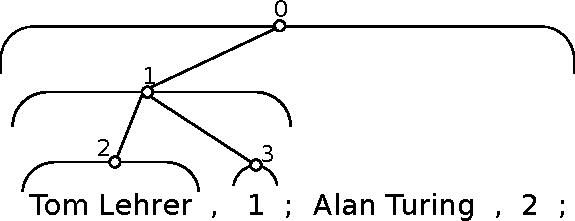
\includegraphics[width=.75\linewidth]{graphs/posix_parse}
\caption{Parse tree produced by \textsc{posix} compatible matching.}
\end{figure}

With our algorithm we are able to reconstruct the full parse
tree after the matching phase is done:

\begin{figure}[h]
\centering
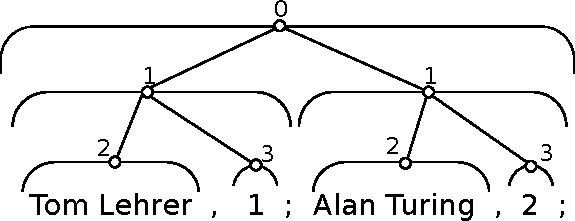
\includegraphics[width=.75\linewidth]{graphs/full_parse}
\caption{Parse tree produced by our approach.}
\end{figure}

The amortized run time of our approach is $O(m\: n)$, where $m$
is the length of the regular expression and $n$ is the length of
the parsed string. This is asymptotically as fast as the best matchers
that don't extract parse trees. 

\subsection{Motivation}

This is the age of big data, and the first step of processing big
data is often to parse strings. As an example, consider log files.
What makes data huge is typically repetition. As Jacobs\cite{Jaco09a}
noted, ``What makes most big data big is repeated observations over
time and/ or space,'' and thus log files grow large frequently. At
the same time, they provide important insight into the process that
they are logging, so their parsing and understanding is important. 

Regular expressions make for scalable and efficient lightweight parsers.\cite{Kart96a} 

The parsing abilities of regular expression have evoked Meiners to declare
that for intrusion detection, ``fast and scalable RE matching is
now a core network security issue.'' \cite{Mein10a}

For example, Arasu et al. \cite{Aras12a} demonstrate how regular
expressions are used in Bing to validate data, by checking whether
the names of digital cameras in their database are valid.

Parsers that can return abstract syntax trees are more useful than
ones that only give a flat list of matches. Of course only regular
grammars can be matched by our approach.

Let us recall what NFAs and DFAs are. A DFA is a state machine that
will walk over the transition graph, one step for every input
character. The choice of transition is limited by the transition's
character range. A transition can only be followed if the current
input character is inside transition's character range. NFAs differ
from DFAs in that for some input character and some state, there may
be more than \ins{one} applicable transition. If there is, an NFA will magically
guess the correct one. \autoref{fig:example-automaton} shows an example of
an NFA's transition graph. For the moment, let us discuss regular
expression matching on NFAs. Assuming that the NFA just magicly knows
the right transition lets us focus on the important things, greediness control
and capture groups.

\section{Algorithm}

Conceptually, our approach is the following pipeline of four stages.
\begin{enumerate}
  \item Parse the regular expression string into an AST.
  \item Transform the AST to an NFA.
  \item Transform the NFA to a DFA.
  \item Compactify the DFA.
\end{enumerate}

In reality, things are a little more involved, since the transformation
to DFA is lazy, and the compactification only happens after no lazy
compilation occurred in a while. Worse, compactification can be
undone if needed. We'll get back to these details in TODO LATER.
Let's discuss the stages in turn, starting with 2, since step 1,
the parsing of the regular expression grammar, is reasonably
straightforward.


\subsection{Thompson's construction} 

We transform the AST of the regular expression into an NFA,
in a modified version of Thompson's NFA construction. To
control greedines, or discern capture groups, our approach adds
$\epsilon$ transitions to the transition graph. An
$\epsilon$-transition has no input range assigned, and can thus always
be used. It does not consume an input character.
The additions are needed for greediness control and capture groups.
Let's look at both, in turn.

To see the importance of greediness control, consider again the regular
expression \texttt{((.*?),(\textbackslash{}d+);)+}. The question
mark sets the \texttt{.*} part of the regular expression to
\emph{non-greedy}, which means that it will match as little as
possible while still producing a valid match, if any.  Without
provisioning \texttt{.*} to be non-greedy, a matching against input
\texttt{``Tom Lehrer,1;Alan Turing,2;''} would match as much as
possible into the first capture group, including the record separator
`,'.  Thus, the first capture group would suddenly contain only one
entry, and it would contain more than just names, namely``Tom
Lehrer,1;Alan Turing''.  This is, of course, not what we expect.
Non-greediness, here, ensures that we get ``Tom Lehrer'', then
``Alan Turing'' as the matches of the first capture group.

In the NFA, we model greedy repetition or non-greedy repetition of
an expression as follows.  First, we construct an NFA graph for the
expression, without any repetition.  We can see how this plays out
in our running example, which contains the expression \texttt{.*?}.
First, an automaton for \texttt{.} is constructed.  As we can see
in \autoref{fig:example-automaton}, expression \texttt{.} is modeled as
just two nodes labeled 3 and 4, and a transition labeled ``any''
between them.  Repeating is achieved by adding two $\varepsilon$
transitions: one from 4 back to 3, to match more than one time any
character, and another one from 3 to 4, to enable matching nothing
at all.  Importantly, the transition from 4 back to 3 is marked as
low priority, while the transition leaving the automaton, from 4
to 5, is unmarked, which means normal priority.  This means that
the NFA will prefer leaving the repeating expression, rather than
staying in it.  If the expression were greedy, then we would mark
the transition from 4 to 5 as low-priority, and the NFA would prefer
to match any character repeatedly.

More generally, the NFA will prefer to follow transitions of normal
priority over those of low priority. Rather than formalize this
notion of preference on NFAs, we come back to prioritized edges when
discussing the transformation from NFA states to DFA states.


\begin{figure*}[tb]
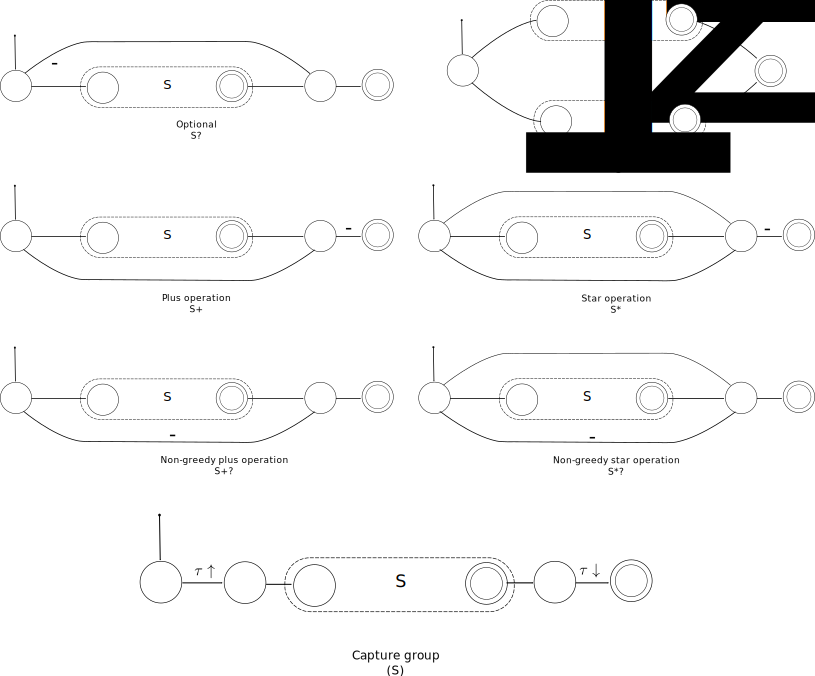
\includegraphics[width=\linewidth]{graphs/thompson}
\caption{Modified Thompson~\cite{Thom68a} construction of the automaton: Decent into the abstract syntax tree of the regular expression and expand the constructs recursively.}
\label{fig:thompson-construction}
\end{figure*}

To model capture groups in the NFA, we add \emph{commit tags} to the
transition graph. The transition into a capture group is tagged by a
commit, the transition to leave a capture group is tagged by a another
commit. We distinguish opening and closing commits. The NFA keeps a
history for every transition with a commit. Each time the transition
is walked, the current position is added to its history. 

We model histories as linked list, where the payload of each node
is a position.  Only the payload of \emph{head}, the first node,
is mutable, the \emph{rest}, all other nodes, are immutable.  Because
the rests are immutable, they may be shared between histories.  This
is an application of the flyweight pattern, and ensures that all
of the following instructions on histories can be performed in
constant time. Here, the \emph{position} is the current position
of the matcher.  It is well-defined at all times since all threads
are executed in lock-step, such that at any point in time, all
threads are at the same position.

\global\long\def\naturals{\mathbb{N}}
\global\long\def\integers{\mathbb{Z}}
\global\long\def\pos{\mathbf{\mathbf{p}}}

\subsection{Instructions of the virtual machine}
\label{instructions}
\begin{description}
\item [$h\leftarrow\pos$] Stores the current position into the head of the linked list $h$.
\item [$h\leftarrow\pos+1$] Stores the position after the current one into the head of linked list $h$.
\item [$h\leftarrow h'$] Sets head->next of $h$ to be head->next of $h'$. 
	This effectively copies the (immutable) rest of $h$ to be the rest of $h'$, also. 
\item [$c\uparrow(h)$] $c\downarrow(h)$ Prepends linked list $h$ with an extra node, which becomes the new head.
This effectively \emph{commits} the old head, which is henceforth considered immutable.
\end{description}

It is easy to see that, after matching, given the history of every tag, the entire match tree can be reconstructed.

\begin{figure}
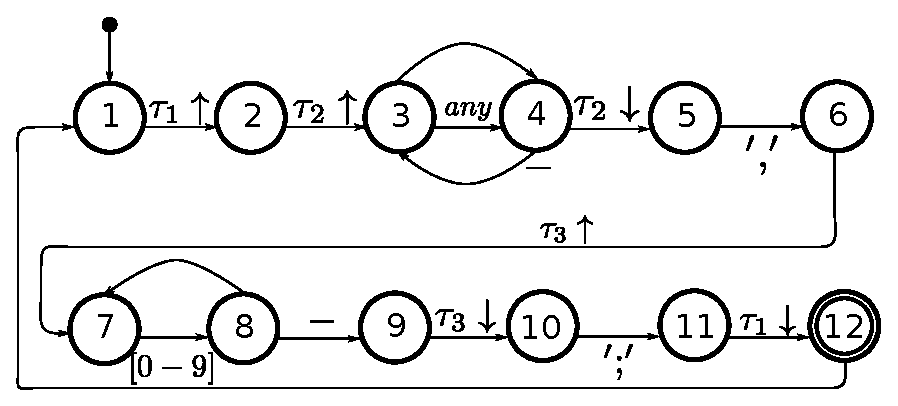
\includegraphics[width=\linewidth]{graphs/lehrer_automaton}

\caption{\label{fig:example-automaton}
Automaton for \texttt{((.*?),(\textbackslash{}d+);)+} 
In the diagram, ``$-$'' stands for low priority. $\tau_n\uparrow$ is the opening tag for capture group $n$, likewise, $\tau_1\downarrow$ is the closing tag for capture group $n$.}
\end{figure}

\subsection{DFAs}

Our above definition of regular expression assumes a machine that
guesses the correct transition through magic. To implement regular
expression matching without supernatural intervention, we lazily transform
the NFA to a DFA. 

A useful metaphor for regular expression matching is that of threads
\cite{Cox07a}. Whenever we aren't sure which transition to take,
we ``fork'' a thread for every option that we have. This way, when
the input is over, there must be at least one thread that guessed
correctly at all times. We use the word ``thread'' here to guide
intuition only. Our approach is not parallel. 

The key insight is that we keep all ``threads'' in lock-step. To
achieve this, we must be very specific about what constitutes the
state of a thread. Since every thread effectively simulates a different
NFA, the state inside of a thread contains exactly two items: the
NFA state it simulates and the history for every tag. Now, the following
would be a correct, although slow, implementation of a non-magic NFA
interpreter: whenever an input character is read, we can iterate over
all threads, kill the ones that have no legal transition for the input
character, and fork more threads as needed.

Trouble starts when we want to fork a thread for an NFA state that
is already running. Not only is an explosion of threads bad for
performance, it would also lead to ambiguity: if the two threads
disagree on the histories, which one is correct?

Algorithm~\ref{onestep}  takes as an input a set of threads, an NFA
transition graph, and an input character, and returns the set of threads
running after the input character has been read. It makes sure that
if there could be two threads with the same NFA state, the one that
follows greedy matching\footnote{Non-greedy operators work the same way, just
with reversed priorities} will survive. At no point of the algorithm are the
two states both present in the result and thus in conflict. This is avoided
by prioritizing the edge with the result that follows the greedy match and
not considering states visited before, ensuring the greedy thread 
``wins the race''.

The following examples will illustrate the algorithm~\ref{onestep} and use the
following notation:

\begin{itemize}
	\item 	A NFA state is denoted as $q_i$.
	\item 	A history is denoted $h_i$. Since a history is actually a
			list of positions in the matched string, we will write it
			as $h_i=[x_1, \dots, x_n]$ to describe that past matches occurred
			at the positions $x_1, \dots, x_n$.
	\item	Each NFA state has an array of $2n$ histories, where 
			$n$ is the number of capture groups in the original 
			regular expression. This is written as 
			$(h_1, h_2, \dots h_{2n-1}, h_{2n})$. The $2i$th 
			position is the history of the opening positions of
			the capture group $i$, the $2i+i$th is the closing position.
			A NFA state of the regular expression \texttt{(.+)} therefore
			has the histories $(h_1, h_2)$ and when matching ``ab''
			$h_1=[0]$ and $h_2=[2]$.
	\item	Each DFA state is denoted by $Q$ and contains multiple NFA 
			states with their current histories. 
			\[Q=\{(q_1, (h_1, h_2, h_3, h_4)), (q_2, (h_1, h_2, h_5, h_6))\}\] for
			example means that the current DFA state has one thread in $q_1$ with 
			histories $(h_1, h_2, h_3, h_4)$ and another in $q_2$ with the histories
			$(h_1, h_2, h_5, h_6)$. Note that histories can be shared across threads
			if they have the same matches.
	\item	A transition is understood to be between NFA states, $1\rightarrow 2$
			means a transition from $q_1$ to $q_2$. The meta-data about the 
			transition is described in the text and can contain consumption
			of characters, priority or opening and closing commit tags.
	\item	The algorithm uses $high$ and $low$ as stacks and \emph{push} means
			to put an element at the topmost position. \emph{Popping} 
			means to remove and retrieve the topmost element of the stack.
	\item	In the examples we will pretend for clarity that the commands
			described in \ref{instructions} are executed directly after they
			are encountered. The actual algorithm collects them and executes 
			them after the $oneStep$ call to allow further optimizations.
\end{itemize}

\begin{algorithm*}[tb]
\SetKwInOut{Input}{Input}\SetKwInOut{Output}{Output}
\DontPrintSemicolon
\SetAlgoLined
\Input{Graph of transitions for an NFA,\\
	   Input character $a$,\\
	   Input position $pos$,\\
	   a set of threads $Q = {(q, [h_{1},\dots,h_{n}])}$,
	     where $q$ is an NFA and $[h_{1},\dots,h_{n}]$ is an array of histories.}
\Output{ Set of threads $R$.}
\Begin{

$R\leftarrow\{\}$\;
Initialize empty stack $low$\;
Initialize empty stack $high$\;

\tcp{1. push follow states with old histories.}
\ForEach{$a$-consuming transition $t$ from any NFA state $q$ to $q'$ such that $(q, H) \in Q$}{
	\lIf{$t$ has low priority}{push $(q', H)$ to $low$ \lElse to $high$}
}

\tcp{2. Follow $\varepsilon$-transitions}
\While{$high$ and $low$ are not both empty}{
	\lIf{possible}{pop $(q', [h_{1},\dots,h_{n}]$ from $high$ \lElse else from $low$\;}
	\lIf{$(q', H) \in R$ for some $H$}{ continue while \;}
	add $(q', [h_{1},\dots,h_{n}])$ to $R$\;
	\ForEach{$\varepsilon$-transitions $t$ from $q'$ to $q''$}{
		\lIf{$(q'', H) \in R$ for some $H$}{continue for loop\;}
		\If{$t$ is tagged with an open or close tag}{
			Choose $i$ such that $h_{i}$ is the history of  $t$'s open tag\;
			Make a new history $h'$\;
			$h'\leftarrow h_{i}$ \label{algline:old-copy}\tcp*{Copy old history}
			\eIf{$t$ has a open tag}{
				Let $newHistories$ be $[\dots,h_{i-1},h',h_{i+1},\dots]$\;
				$h' \leftarrow pos+1$ \label{algline:store-after}\tcp*{Store position after current}
			}{
			\tcp{$t$ has a close tag}
			Choose $i'$ such that $h_{i'}$ is the history of  $t$'s open tag \;
			Make a new history $h''$\;
			$h'' \leftarrow h_{i'}$ \label{algline:old-copy2}\tcp*{Copy old history}
			$h'' \leftarrow pos$\label{algline:store-current}\tcp*{Store current position}
			Commit $h'$\;
			Commit $h''$\;
			Let $newHistories$ be $[\dots,h_{i-1},h', \dots, h'',h_{i'+1},\dots]$\;
			}
		}
					
				
		\tcp{Push according to priority of transition:}
		\lIf{$t$ has low priority}{push $(q'', newHistories)$ to $low$, \lElse to $high$}
	}
}
}

\caption{\label{onestep}$oneStep(NFA, a, pos, Q)$: Compute the follow-up state for DFA state $Q$}
\end{algorithm*}


\begin{algorithm*}[h]
\SetKwInOut{Input}{Input}\SetKwInOut{Output}{Output}
\DontPrintSemicolon
\SetAlgoLined
\Input{$input$ is a sequence of characters}
\Output{a tree of matching capture groups for the regex}
\Begin{
\tcp{Lazily compiles a DFA while matching.}

Set $Q$ to startState.\;
\tcp{A thread is an NFA state, with an array of histories.}
Let $Q$ be all threads that are reachable in the NFA transition graph by following $\varepsilon$ transitions only.\;
Execute instructions described in $oneStep$ when walking $\varepsilon$ transitions.\;

\tcp{Create the transition map of the DFA.}
Set $T$ to an empty map from state and input to new state and instructions.
\;
\tcp{Consume string}
\ForEach{position $pos$ in $input$}{
	Let $a$ be the character at position $pos$ in $input$.
	
	\eIf{$T$ has an entry for $Q$ and $a$}{
		// Let the DFA handle $a$
		Read the instructions and new state $Q'$ out of $T$\;
		execute the instructions\;
		$Q\leftarrow Q'$\;
		jump back to start of for loop.\;
	}{ %else
		\tcp{lazily compile another DFA state.}
		Run $oneStep(Q,a)$ to find new state $Q'$ and instructions \;
		Run $findMapping(Q', T)$ to see if Q' can be mapped to an existing state $Q''$\;
		\eIf{$Q''$ was found}{
			Append the mapping instructions from $findMapping$ to the instructions found by $oneStep$\;
			Execute the instructions.\;
			Add an entry to $T$, from current state $Q$ and $a$, to new state $Q''$ and instructions.\;
			Set $Q$ to $Q''$\;
		}{ %else
			Execute the instructions found by oneStep.\;
			Add an entry to $T$, from current state $Q$ and $a$, to new state $Q'$ and instructions.\;
			Set $Q$ to $Q'$.\;
		}
	}

}
}
\caption{$interpret(input)$: Interpretation and lazy compilation of the NFA
\on{This looks really horrible monospaced -- please don't use the listings package here!}}
\end{algorithm*}

\begin{algorithm*}[h]
\SetKwInOut{Input}{Input}\SetKwInOut{Output}{Output}
\DontPrintSemicolon
\SetAlgoLined
\Input{$Q=\{(q_i, h_i)\}_{i=1\dots n}$ is a DFA state.}
\Output{A state $Q'$ that $Q$ is \emph{mappable} to.\\
	The ordered instructions $m$ that reorder the memory 
		locations of $Q$ to $Q'$ and don't interfere with each other.}
\Begin{
    
\ForEach{ $Q'$ such that $\{q_i\} = \{q'_i\}$}{

	\tcc{Invariant: For each history $H$ there is at most one $H'$\\ so that $H\leftarrow H'$ is part of the mapping.}
	Initialize empty map $m$\;
	
	\ForEach{$q_i=q'_i$ with histories $H$ and $H'$ respectively}{
		\For{$i=0\dots length(H)-1$}{
    
			
			\eIf{$H(i)$ is in $m$ as a key already and does not map to $H'(i)$}{
				Fail\;
			}{
			
				Add $H'(i)\leftarrow H(i)$ to $m$ \tcp*{Hypothesize that this is part of a valid map}
				}
			}
		}
    }
	\tcp{The mapping was found and is in $m$ if we didn't fail.}
  
	sort $m$ in reverse topological order so that no values are overwritten. \;
  
	\Return{$Q'$ and $m$}
}
\caption{$findMapping(Q)$: Finding a state that $Q$ is mappable to in order to keep the number of states created bound by the length of the regular expression.}
\end{algorithm*}

\begin{example} Execution of algorithm \ref{onestep}:
\label{ex:oneStep1}

Assume as an example the automaton in figure \ref{fig:example-automaton} is in the DFA state\footnote{NFA states that do not have any outgoing transitions except for $\varepsilon$ transitions can be omitted, since the first step will only consider edges which consume the next character of the input.} 
\begin{align*}
Q=\{
	(q_3, (&h_1=[0], h_2=[0], h_3=[0], \\
	&h_4=[0], h_5=[0], h_6=[0])), \\
	(q_5, (&h_1=[0], h_2=[0], h_7=[0,0], \\
	&h_8=[0,0], h_5=[0], h_6=[0]))\}
	\end{align*}
\on{I don't know how to read this.  What does this mean?}
This is the case after initialization or before any commas are read.

This is the execution of $oneStep(NFA, ``a'', 1, Q)$:

\begin{enumerate}
\item Initialize $high$ and $low$ as empty stacks.
\item Initialize $R=\{\}$
\item The only transition that consumes ``a'' is $3\rightarrow 4$. $(4, (h_1, h_2, h_3, h_4, h_5, h_6))$ is pushed to $high$ \on{What's $high$? What are $h_1$ etc?}
\item $(4, (h_1, h_2, h_3, h_4, h_5, h_6))$ is popped from $high$. \on{What does it mean to push/pop?}
\item $R=\{(4, (h_1, h_2, h_3, h_4, h_5, h_6))\}$
\item $4\rightarrow 3$ is visited. \begin{enumerate}
	\item $(3, (h_1, h_2, h_3, h_4, h_5, h_6))$ is pushed to $low$.
\end{enumerate}
\item $4\rightarrow 5$ is visited. \begin{enumerate}
	\item A new history $h_9$ is created.
	\item $h_9\leftarrow h_3$ is executed -- we copy the head and the tail of $h_3$ into $h_9$, so that they can change independently. \on{huh?}
	\item A new history $h_{10}$ is created.
	\item $h_{10}\leftarrow h_4$ is executed.
	\item $h_{10} \leftarrow 1$ is executed. \on{huh?}
	\item Commit $h_9$. It is now $h_9=[0,0]$. \on{Still don't know what this means}
	\item Commit $h_{10}$. It is now $h_{10}=[1,1]$.
	\item $(5, (h_1, h_2, h_9, h_{10}, h_5, h_6))$ is pushed to $high$.
\end{enumerate}
\item No further transitions are visited from $4$.
\item $(5, (h_1, h_2, h_9, h_{10}, h_5, h_6))$ is popped from $high$.
\item $R=\{(4, (h_1, h_2, h_3, h_4, h_5, h_6)),\allowbreak (5, (h_1, h_2, h_9, h_{10}, h_5, h_6))\}$
\item No transitions are visited from $5$.
\item $(3, (h_1, h_2, h_3, h_4, h_5, h_6))$ is popped from $low$.
\item $3\rightarrow 4$ is visited \begin{enumerate}
	\item $4$ is in $R$, so no further steps are taken.
\end{enumerate}
\item No further transitions are visited from $3$.
\item Both stacks are empty, $R$ is returned.
\end{enumerate}
\end{example}


\begin{example} Execution of algorithm \ref{onestep} with an ambiguous consumption:

Take the NFA as above and 
\begin{align*}
Q=\{
	(q_3, (&h_1=[0], h_2=[0], h_3=[0], \\
	&h_4=[0], h_5=[0], h_6=[0])),\\
	(q_5, (&h_1=[0], h_2=[0], h_7=[1,1],\\ 
	&h_8=[1,1], h_5=[0], h_6=[0]))\}
\end{align*}

This is the execution of $oneStep(NFA, ``,'', 2, Q)$:
\begin{enumerate}
\item The character ``,'' can be consumed by the transition $5\rightarrow 6$ and the transition $3\rightarrow 4$.
\item $(6, (h_1, h_2, h_7, h_8, h_5, h_6))$ is pushed to the stack $high$
\item $(4, (h_1, h_2, h_3, h_4, h_5, h_6))$ is pushed to the stack $high$
\item $(4, (h_1, h_2, h_3, h_4, h_5, h_6))$ is popped from $high$.
\item $R=\{(4, (h_1, h_2, h_3, h_4, h_5, h_6))\}$
\item $4\rightarrow 3$ is visited. \begin{enumerate}
	\item $(3, (h_1, h_2, h_3, h_4, h_5, h_6))$ is pushed to $low$.
\end{enumerate}
\item $4\rightarrow 5$ is visited. \begin{enumerate}
	\item A new history $h_9$ is created.
	\item $h_3\rightarrow h_9$ is executed.
	\item A new history $h_{10}$ is created.
	\item $h_4\rightarrow h_{10}$ is executed.
	\item $h_{10} \leftarrow 1$ is executed.
	\item Commit $h_9$. It is now $h_9=[0,0]$.
	\item Commit $h_{10}$. It is now $h_{10}=[1,1]$.
	\item $(5, (h_1, h_2, h_9, h_{10}, h_5, h_6))$ is pushed to $high$.
\end{enumerate}
\item No further transitions are visited from $4$.
\item $(5, (h_1, h_2, h_9, h_{10}, h_5, h_6))$ is popped from $high$.
\item $R=\{(4, (h_1, h_2, h_3, h_4, h_5, h_6)),\allowbreak (5, (h_1, h_2, h_9, h_{10}, h_5, h_6))\}$
\item No transitions are visited from $5$.
\item $(6, (h_1, h_2, h_3, h_7, h_8, h_5, h_6))$ is popped from $high$.
\item $R=\{(4, (h_1, h_2, h_3, h_4, h_5, h_6)),\allowbreak (5, (h_1, h_2, h_9, h_{10}, h_5, h_6)),\allowbreak (6, (h_1, h_2, h_3, h_7, h_8, h_5, h_6))\}$
\item $6\rightarrow 7$ is visited.\begin{enumerate}
	\item A new history $h_{11}$ is created.
	\item $h_5\rightarrow h_{11}$ is executed.
	\item $(7, (h_1, h_2, h_7, h_8, h_{11}, h_6))$ is pushed to $high$.
\end{enumerate}
\item No further transitions are visited from $6$.
\item $(7, (h_1, h_2, h_7, h_8, h_{11}, h_6))$ is popped from $high$.
\item No transitions are visited from $7$.
\item $(3, (h_1, h_2, h_3, h_4, h_5, h_6))$ is popped from $low$.
\item $3\rightarrow 4$ is visited \begin{enumerate}
	\item $4$ is in $R$, so no further steps are taken.
\end{enumerate}
\item No further transitions are visited from $3$.
\item Both stacks are empty, $R$ is returned.
\end{enumerate}
\label{ex:oneStep2}
\end{example}

Our algorithm ensures that the compilation of the regular expression 
terminates by implementing the mapping scheme from \cite{Laur00a}. 
Mappings are best understood as an optimization that allows reuse
of DFA states, that are ``similar enough''. DFA states that have the 
same structure can be reused. For example the DFA state 
$Q=\{(q_1, (h_1, h_2))\}$ is structurally no different from 
$Q'=\{(q_1, (h_3, h_4))\}$. Instead of creating a new DFA state $Q'$ 
in the automaton, we can simulate it by a transition to $Q$ with the
added instructions $h_1\leftarrow h_3$ and $h_2 \leftarrow h_4$.

\begin{example} Executing $findMapping$:

After the execution seen in example~\ref{ex:oneStep1} the new proposed state is 
\begin{align*}
Q'=\{(q_4, (&h_1=[0], h_2=[0], h_3=[0], \\
	&h_4=[0], h_5=[0], h_6=[0])), \\
	(q_5, (&h_1=[0], h_2=[0], h_9=[0,0],\\
	& h_{10}=[1,1], h_5=[0], h_6=[0]))\}
\intertext{and the previous DFA state was}
Q=\{(q_3, (&h_1=[0], h_2=[0], h_3=[0],\\
	&h_4=[0], h_5=[0], h_6=[0])),\\
	(q_5, (&h_1=[0], h_2=[0], h_7=[0,0],\\
	&h_8=[0,0], h_5=[0], h_6=[0]))\}
\end{align*}

This is the execution of $findMapping(Q', DFA)$: 
\begin{enumerate}
\item $Q$ is considered as a candidate
\item $q_3$ is checked \begin{enumerate}
	\item All histories can be mapped with the identity.
\end{enumerate}
\item $q_5$ is checked \begin{enumerate}
	\item $h_1, h_2, h_5, h_6$ can be mapped with the identity.
	\item $h_9$ can be mapped to $h_7$.
	\item $h_{10}$ can be mapped to $h_8$.
\end{enumerate}
\item The mapping is successful and the instructions $h_8 \leftarrow h_{10}$ and $h_7 \leftarrow h_9$ are returned.
\end{enumerate}
Note that by construction at most one candidate fulfils the requirement that the same states are present.
\end{example}
\section{TDFA with commits\label{sec:TNFA-with-hierarchical}}
DEPRECATED

The overall idea is simple: whenever the TDFA is reading in a run
of characters that belong to a capture group, we push the previous
one into our history and the work on current one. To implement this,
we introduce ``commits'' into the TDFA. On the level on the TNFA
the commits correspond to tags at the end of capture groups. Since
capture groups are nested, they form a tree. We will call this three
the match tree and will prove that we can reconstruct it. In it, we
store all runs that this capture group matches. The subnodes of a
hierarchy nodes correspond to the submatches of its capture group.We
will shortly discuss how to construct a TDFA that includes instructions
that \emph{commit} submatches into the hierarchy nodes.. Once we have
the instructions, during interpretation of the TDFA, whenever we encounter
an input character that closes a capture group, the TDFA will \emph{commit}
that capture group. To commit a substring into a hierarchy node has
the following semantics.

A hierarchy node, as a tree node, has a corresponding subtree. The
data in this subtree represents precisely the subtree of the AST that
is currently being matched. Upon commit of the hierarchy node, it
constructs this AST subtree, and stores it as a previous match. Iteratively,
this produces all matches of all capture groups.

\begin{comment}
if the current set of characters compare the current reading with
the previously longest read, keeping the longer one. n order to get
some more control over the overwriting of the tags, a separate \texttt{commit}
step can be introduced. Each nesting then would need a separate copy
of the temporary ``best'' match for a given group. For example \texttt{(((a+)b)+c)+}
would need two additional copies of the innermost group, to handle
conflicts. 

The intuition is to notice that two tags -- the opening and the corresponding
end tag -- always appear in order and the inner groups should not
spill over the end of the outer group. After each closing tag then
a commit is made, which handles whether the new or the old match is
longer. 
\end{comment}

\begin{figure}
\begin{centering}
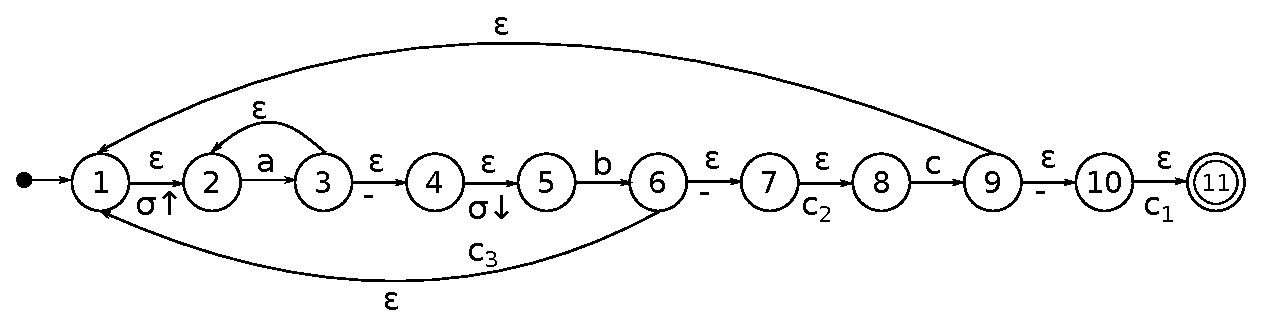
\includegraphics[width=\linewidth]{graphs/abc}
\par\end{centering}

\caption{NFA about to be transformed.}
\end{figure}
In the following, the regex \texttt{(((a+)b)+c)+} will be converted
to a \textsc{dfa} lazily while matching the string ``abaababc'',
the resulting DFA can be seen in \ref{fig:lazy-dfa}: 
\begin{enumerate}
\item The starting state is $(1[-1,-2],2[0,-2])$ and the memory location
$0$ is initialized to hold the index $0$.
\item Now the letter a is read:

\begin{enumerate}
\item $2[0,-2]$ leads to $3[0,-2]$
\item $3[0,-2]$ leads to $2[0,-2]$
\item $3[0,-2]$ leads to $4[0,-2]$
\item $4[0,-2]$ leads to $5[0,1]$, with the instruction to write the index
to $1$ and commit the memory locations $(0,1)$ on level $3$ afterwards.
The hierarchical memory is now $c_{1}=nil,c_{2}=nil,c_{3}=(0,1)$,
where $(0,1)$ are the indeces, not the memory locations.
\end{enumerate}
\item Next the letter b is read:

\begin{enumerate}
\item $5[0,1]$ leads to $6[0,1]$
\item $6[0,1]$ leads to $1[0,1]$
\item $1[0,1]$ leads to $2[2,1]$, with the instruction to write the current
index to $2$.
\item $6[0,1]$ leads to $7[0,1]$
\item 7{[}0,1{]} leads to $8[0,1]$, with the instruction to commit to the
second level. The hierarchical memory is now $c_{1}=nil,c_{2}=(0,1),c_{3}=(0,1)$.
\end{enumerate}
\item Next the letter a is read:

\begin{enumerate}
\item $2[2,1]$ leads to $3[2,1]$
\item $3[2,1]$ leads to $2[2,1]$
\item $3[2,1]$ leads to $4[2,1]$
\item $4[2,1]$ leads to $5[2,3]$, with the instruction to write the current
index to memory location $3$ and commit the third level: $c_{1}=nil,c_{2}=(0,1),c_{3}=(2,3)$
\item We find, that this state is mappable to the previous state $(2[0,-2],3[0,-2],4[0,-2],5[0,1])$
with the mapping $2\rightarrow0,1\rightarrow-2$.
\end{enumerate}
\item Next the letter a is read:

\begin{enumerate}
\item $2[0,-2]$ leads to $3[0,-2]$
\item $3[0,-2]$ leads to $2[0,-2]$
\item $3[0,-2]$ leads to $4[0,-2]$
\item $4[0,-2]$ leads to $5[0,1]$, with the instruction to write the current
index to memory location $1$ and commit the third level: $c_{1}=nil,c_{2}=(0,1),c_{3}=(2,4)$.
\end{enumerate}
\item Next the letter b is read, but the transition is already known:

\begin{enumerate}
\item We write the current index into memory location $2$ and commit the
second level. Now the match $(2,4)$ is compared against the previous
match $(0,1)$, but the length of the new match is bigger, therefore
the new match overwrites the old one. $c_{1}=nil,c_{2}=(2,4),c_{3}=(2,4)$.
\end{enumerate}
\item Next the letter a is read, but the transition is already known:

\begin{enumerate}
\item We write the current index into memory location $-2$ (because of
the mapping) and commit $(2,-2)$ to the third level. $c_{1}=nil,c_{2}=(2,4),c_{3}=(5,6)$.
\end{enumerate}
\item Next the letter b is read, but the transition is already known:

\begin{enumerate}
\item We write the current index into memory location $2$ and commit to
the second level. The match $(5,6)$ is compared against the previous
match $(2,4)$, but the length of the old match is bigger, therefore
the old match is kept. $c_{1}=nil,c_{2}=(2,4),c_{3}=(5,6)$.
\end{enumerate}
\item Next the letter c is read:

\begin{enumerate}
\item $8[0,1]$ leads to $9[0,1]$
\item $9[0,1]$ leads to $1[0,1]$
\item $1[0,1]$ leads to $2[2,1]$, with the instruction to write the current
index to memory location $2$.
\item $9[0,1]$ leads to $10[0,1]$)
\item $10[0,1]$ leads to $11[0,1]$, with the instruction to commit to
the first level. $c_{1}=(2,4),c_{2}=(2,4),c_{3}=(5,6)$.
\end{enumerate}
\item Finally the end of the string is read.

\begin{enumerate}
\item We are in a finishing state $11[0,1]$, therefore the match succeeds.
The current commit of the top layer is returned: $c_{1}=(2,4)$.
\end{enumerate}
\end{enumerate}
\begin{figure}
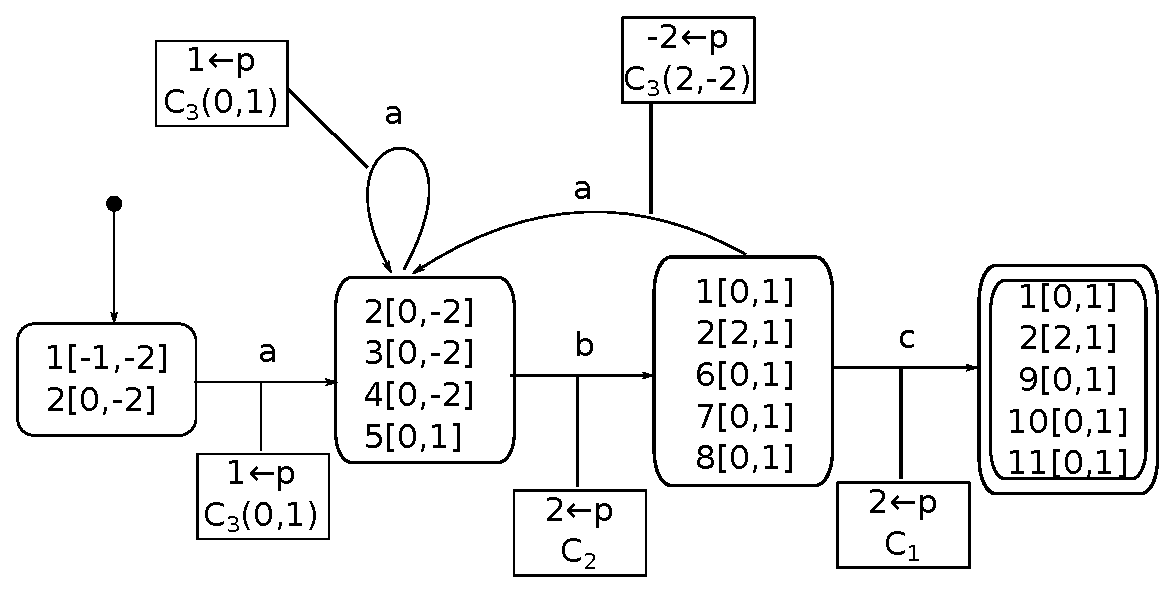
\includegraphics[width=\linewidth]{graphs/abc-dfa}

\caption{\label{fig:lazy-dfa}The DFA of \texttt{(?:(?:(a+)b)+c)+} matching
``abaababc''}


\end{figure}
\begin{comment}
This technique allows for programmers to extract parts of text with
great performance and flexibility regarding the extracted match. One
could imagine, that a programmer needs to extract a ideally complete
sample of formated text with optional parameters. Here, \texttt{\textsc{posix}}
regex would fail to deliver the best match in most cases. Such cases
can occur in data mining, in bioinformatics, both of which are handling
massive data, so that efficiency can be a problem.
\end{comment}


\section{Benchmark}


\section{Related work}
Our algorithm is a modification of Laurikari's algorithm \cite{laurikari2000nfas},
which is itself a modified powerset construction algorithm \cite[p. 55]{Sipser2005}.

While there is no shortage of books discussing the usage of regular
expressions, the implementation side of regular expression has not
been so lucky. Cox is spot-on when he argues that innovations have
repeatedly been ignored and later reinvented \cite{Cox07a}. 

This paper is no exception. The authors of this paper had set out
to implement Laurikari's TDFA algorithm \cite{Lauri00a},
only to discover that Laurikari's description of a TDFA is so far
from complete that it can rightfully only be called the sketch for
an algorithm. Only late in the process did we discover that the blanks
had already been filled by Kuklewicz in the course of his implementation
of TDFAs in Haskell \cite{Kukl07a}. Kuklewicz enshrined his
added insight into Haskell library, but never published the algorithm
as a whole. If the history of regular expressions is evidence of one
thing, it is that source code is a terrible medium to convey algorithms. 

The situation dramatically improved with Cox's simple and concise
explanation of regular expression matching \cite{Cox07a}. It seems
ironic that this well-versed author published his influential work
on his website. Although the joke may be on Academia's side.

When the taciturn practioners acknowledge each other's work, we can't
help but disagree almost universally with the characterizations they
produce. Sulzmann and Lu \cite{Sulz12a} call Kuklewicz's
work an ``implementation'' of Laurikari's algorithm, although Laurikari's
algorithm is far too incomplete for that statement to be fair. Laurikari's
algorithm is referred to as a POSIX-style automaton. In truth, Laurikari
leaves the matching strategy entirely open. It was Kuklewicz that
found out how to get POSIX-style matching out of Laurikari's TDFA. 

Cox says that Laurikari's TDFA is a reinvention Pike's published only
in code algorithm \cite{Pike87a}, which is Thompson's NFA with submatch
tracking. This seems unfair in that Laurikari's allows for far more
aggressive reusing of old states than what Thompson allows. This should
lead to Laurikari's TDFA having fewer states, and therefore better
performance, than even Google's RE2, which uses Pike's algorithm.
This is not confirmed by the benchmarks by Sulzmann and Lu \cite{Sulz12a},
but they offer an explanation: in their profiling, they see that all
Haskell implementations spend considerable time decoding the input
strings. In other words, the measured performance is more of an artifact
of the programming environment used. 

Another mistake that permeates the scarce literature is to call regular
expression matching linear. As Sedgewick points out correctly \cite{Sedg90a},
Thompson's NFA matching is of complexity $O(mn)$, where $m$ is the
size of the input NFA, and $n$ is the size of the input string. To
call this linear requires to assume $m$ to be fix, which we cannot
bring ourselves to justify. It may well be true that, at present,
$m$ tends to be small. But that is a natural consequence of the algorithms
not scaling very well with $m$. If they did, that would allow for
fast feature extracting from text. Therefore, in this paper, we consider
the state of the art algorithms to be quadratic, since both $m$ and
$n$ are part of the input to a regular expression matcher. We cannot
rule out that a linear algorithm exists, in fact, we hope for it.
To insist that regular expression matching is done in linear time
is to insist that the optimal algorithm has already been found; that
is probably not true.

Sulzmann and Lu add to the table a new matching strategy that yields
good practical performance, although the theoretical bounds are considerably
worse than the state of the art, at $O(n^{2}m)$ \cite{Sulz12a}.

\bibliographystyle{plain}
\bibliography{bib/scg}
\end{document}
